\documentclass[conference,letter,10pt,final]{IEEEtran}
\usepackage[utf8]{inputenc}
\usepackage[T1]{fontenc}
\usepackage{fixltx2e}
\usepackage{graphicx}
\usepackage{grffile}
\usepackage{longtable}
\usepackage{wrapfig}
\usepackage{rotating}
\usepackage[normalem]{ulem}
\usepackage{amsmath}
\usepackage{textcomp}
\usepackage{amssymb}
\usepackage{capt-of}
\usepackage{hyperref}
\usepackage[utf8]{inputenc}
\usepackage[T1]{fontenc}
\usepackage{lipsum}
\date{}
\title{Automatic Memory-Bound Phase Detection using Time-oriented Hardware Counters Metrics}
\hypersetup{
 pdfauthor={Gabriel Bronzatti Moro, Lucas Mello Schnorr},
 pdftitle={Automatic Memory-Bound Phase Detection using Time-oriented Hardware Counters Metrics},
 pdfkeywords={},
 pdfsubject={},
 pdfcreator={Emacs 24.3.1 (Org mode 8.3.4)}, 
 pdflang={Pt-Br}}
\begin{document}


\title{Automatic Memory-Bound Phase Detection \\ using Time-oriented Hardware Counters Metrics}

\author{
\IEEEauthorblockN{Gabriel Bronzatti Moro, Lucas Mello Schnorr}
\IEEEauthorblockA{Institute of Informatics, Federal University of Rio Grande do Sul \\
Caixa Postal 15064 –- CEP 91501-970 Porto Alegre -- RS -- Brazil\\}
}

\maketitle

\begin{abstract}
Besides reducing the execution time of parallel applications, the power
consumption is an increasingly addressed problem in High-Performance
Computing. A parallel program may be composed of different
parallel regions, which can have particular characteristics, for instance,
CPU or memory bound. This paper presents an
approach that allows the automated detection of memory-bound parallel
regions. Our approach differs from others found in the literature
because it detects automatically parallel regions that depend more
of the memory, all samples collected from the application did not require
any code instrumentation, advantage of the present work, the
less intrusive possible. The applications used in the experiment
were the Discrete 3D fast Fourier Transform (FT), Lower-Upper
Gauss-Seidel solver and Conjugate Gradient, both of the NAS benchmark
parallel. In the experiment was evaluated the miss rate for the L2
cache. Through of the experiment was possible to identify the memory-bound
regions by timestamps of the applications. The results show that is
possible to identify the memory-bound regions and too the behavior of
applications as a whole. From the knowledge of these regions it is
possible to configure a suitable processor frequency for each parallel
region of the application, reducing the energy used and improving the
performance of the application as a whole. 
\end{abstract}

\section{Introduction}
\label{sec:orgheadline1}

%- Large HPC applications are usually composed by many parallel regions
%- Give some examples

Large HPC applications are composed of parallel regions, these regions
may be regarded program fragments that are executed by different
threads. For example, in an application that calculates heat exchange
in a metal plate, could be considered a problem which has two sets of
parallel regions, the first set calculate the initial state of the
plate and another part would be responsible for calculating the heat
exchange in different points of the plate. In the first set there are
various parallel regions, whether divided in "n" timestamps, it is
possible to see various behaviors, some more memory-bound, others more
CPU-bound. 

%- Each code region has its own memory/cpu/io resource requirements
%- Some might be more memory-bound, others cpu-bound, for example

Each parallel region has its own characteristic, some may be
considered memory-bound, where there is a high rate of the
cache miss, while others may be considered more CPU-bound, which
expects more by CPU resource and more IO-bound when the thread is
limited by waiting for input or output operations. In the previous
example of the heat plate, the second  set of parallel regions can be
considered more memory-bound than the first set, more within of each
set may exists regions with behaviors various.  

%- Automatically detecting such regions could potentially lead to
% per-parallel region improvements such as energy and performance
% improvements by adopting an appropriate processor frequency to
% execute

From an automatic detection of parallel regions of an application it
is possible to adjust the processor to frequency appropriate to the
region, according to its features (memory or CPU bound), which may allow
a reduction in energy consumption and an increase application
performance as a whole.

%- The idea of this work is to measure hardware counters along time in
%  order to correlate their values against the different code region
%  - With this information, we intend to detect memory-bound code
%    regions that could be potential candidates for energy reduction
%    strategies (mainly DVFS)
%  - Once the memory-bound code regions have been detected, we intend
%    to apply Design of Experiments techniques to find the best
%    processor frequency configuration for each region, pretty similar
%    to what has been done already lfgmillani2016reppar, but
%    automatically.

The main objective of this study is to measure hardware counters
specific for each parallel region code to define regions
having more memory-bound behavior, which could be
candidates for strategies to reduce energy consumption (using
Dynamic Voltage Frequency Scaling).

The preliminary results indicate that the technique used in this work
allows automated identification of the memory-bound regions in a
parallel application with a low level of intrusion, different
approaches investigated \cite{freeh2005exploring,millani2006fr}. In
addition to identifying regions, it is also possible to identify the
behavior of the application as a whole based on different hardware
counters.  

%- Paper structure

This paper has the following
organization. Section \ref{sec:relatedwork} presents related work
regarding automatic phase detection for HPC applications. It also
motivates our work. Section \ref{sec:methodology} details our proposal
and its corresponding methodology to fullfill our goal, which is the
automatic phase detection using time-oriented hardware
counters. Section \ref{sec:results} the plataform we have been using
to conduct experiments and the preliminary results we have obtained so
far. Section \ref{sec:conclusion} concludes the paper listing the main
contributions and future work.   

\section{Related Work}
\label{sec:orgheadline2}
\label{sec:relatedwork}

%- There is no definitive solution to detect if a code region is more
%memory or CPU bound.
%- Usually hard. counters are globally aggregated
%- Automatic techniques usually rely on specific hardware counters

There is no definitive solution to detect if a code region is more
memory or CPU bound. The main focus of this work is to characterize
the behavior of code regions of a parallel application, classifying
them into memory and/or CPU bound. For thereafter to be able to find
an appropriate frequency for each region, using DVFS (Dynamic Voltage
Frequency Scaling) technique.

Some works focus more on phase detection to sequential applications
\cite{spiliopoulos2012power}\cite{laurenzano2011reducing}. Spiliopoulos
et al.\cite{spiliopoulos2012power} present in his work a tool that
analyzes the behavior of a sequential application by detailed analysis
of its phases of execution, based on cache misses of the different
levels of cache, the tool identifies the best processor frequency to
be used in each phase to best performance and reduce energy
consumption. In addition to this approach, Laurenzano et
al.\cite{laurenzano2011reducing} present an approach finer granularity
for identifying the most appropriate processor frequency for each loop
of application. From the executions, it is defined a model of multiple
dimensions that allows find given loop frequency that best defines the
behavior of energy and expected performance. 

For parallel applications, there is advances in the detection of
stages for MPI applications \cite{freeh2005exploring}, already to
OpenMP applications, there is one approach that allows the
instrumentation via code to indicate the parallel regions
\cite{millani2006fr}. Freeh et al.\cite{freeh2005exploring} present an 
approach that to provide the most suitable frequency for each phase of
an MPI application, the application of this approach is divided
according to the number of cluster processors used. Among the
available frequencies, the approach looks at what is the best
frequency for a given node operate during the execution of the
application.

An approach that focuses on shared memory applications in OpenMP is
Millani and Schnorr \cite{millani2006fr}. In this work are analyzed
parallel regions of a program, according to the study it is possible
to reach a considerable gain in energy reduction and performance
increase through the use of a suitable frequency for each parallel
region of the program. Also, in this approach the parallel regions are
instrumented, already in our work the parallel regions will be known
during program execution, the level of intrusion of our approach is
lower and it is possible to identify the behavior of the memory-bound
regions and from these reduce the processor frequency, lowering power
consumption and improving performance. 

\section{Methodology}
\label{sec:orgheadline3}
\label{sec:methodology}

The methodology used in the work first defines the compilation a
source code into binary after that to run this program is used to a
likwid-perfctr tool that allows you to collect events each processing
core. These events are processed by a script we created to generate a
detailed trace of the application for make the data analysis. In the
Figure \ref{figMetodologia} it is possible to see an overview of the
methodology.

\begin{figure}[!htb] \label{figMetodologia}
\caption{Overview of the methodology.}
\centering 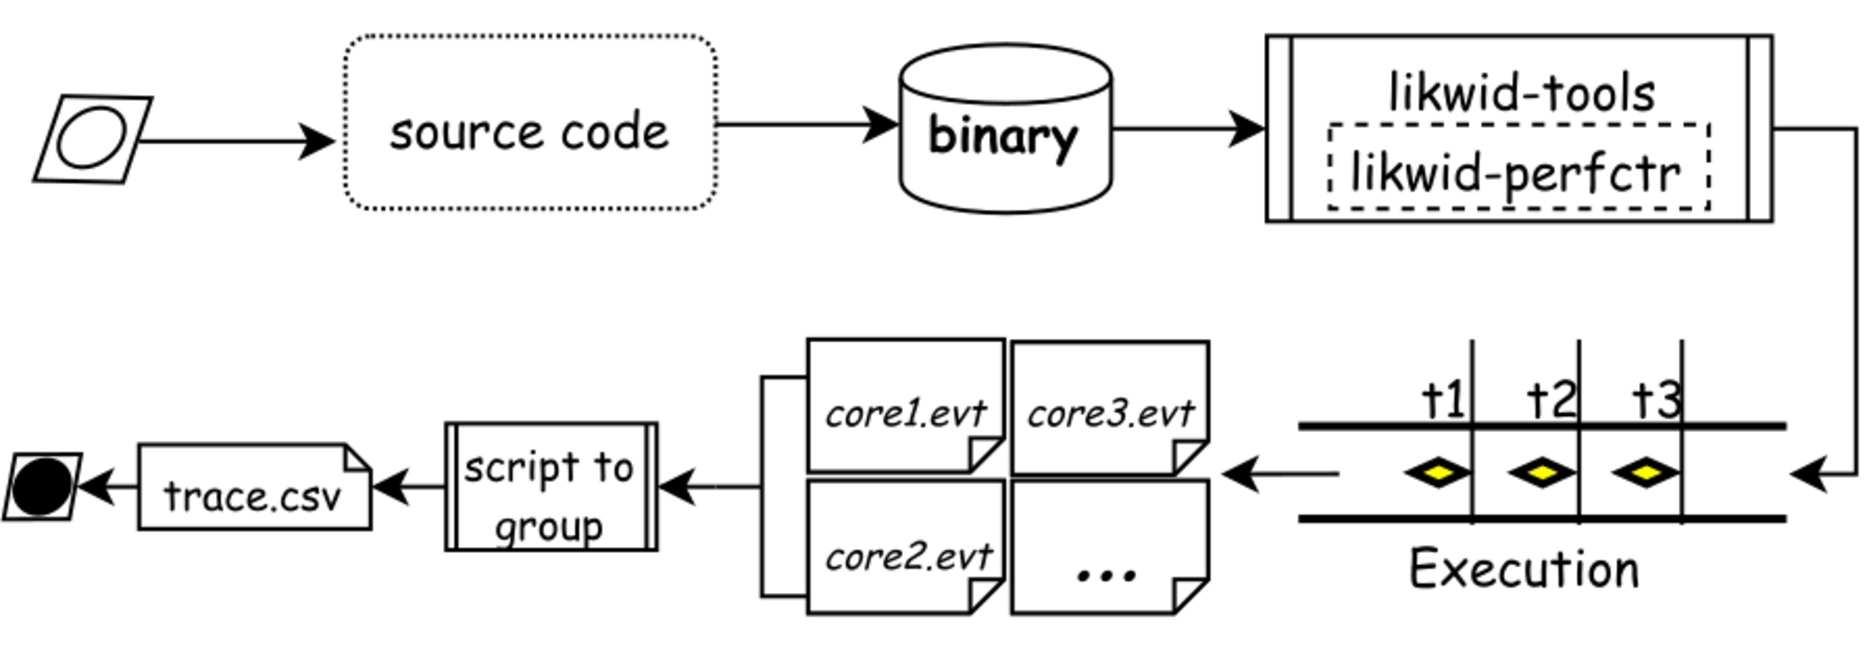
\includegraphics[width=5cm,height=6cm]{img/metodologiaWorkWsppd2016.pdf}
\end{figure}

In the experiment were used OpenMP applications of the NAS Parallel
Benchmarks. These applications were chosen two, the 3D Discrete Fast
Fourier Transform (FT), Lower-Upper Gauss-Seidel Solver (LU) and
Conjugate Gradient (CG), because in them it is possible to see two
very different behaviors in misses rate for the L2 Cache when compared
to other applications of the benchmark. 

The applications were executed with 32 threads, both applications used
the bigger input size (class B) of the benchmark. The execution
platform used was a Workstation with 2 processors Intel (R) Xeon (R)
E5-2650 CPU 2.00 GHz, each with 8 physical cores and Hyper-Threading
technology. 

To understand the behavior of the memory-bounds parallel regions was
used to likwid tool that allowed collecting in each timestamp basic
measures over the miss rate to the L2 Cache. The interval between
timestamps was defined according to the total execution time of each
application. For example, in the FT application, the interval was
between timestamps was 30ms (milliseconds) generating about 172
samples (for each of the 32 threads). Already for the LU application
was defined a wider range of 100ms, which generated about 363
samples. The wider range defined for the CG application was 50ms,
which generated about 384 samples. 

\section{Preliminary Results}
\label{sec:orgheadline4}
\label{sec:results}

The graphs have two lines, the first describes the miss
rate behavior in the L2 and L3 cache to the first processor (socket with
8-physical colors) and the second line to the other processor. Each
point on the graph presents a coordinated, where was a sample
collected on their timestamp. 

\begin{figure}[htp]\label{figFT}
\centering 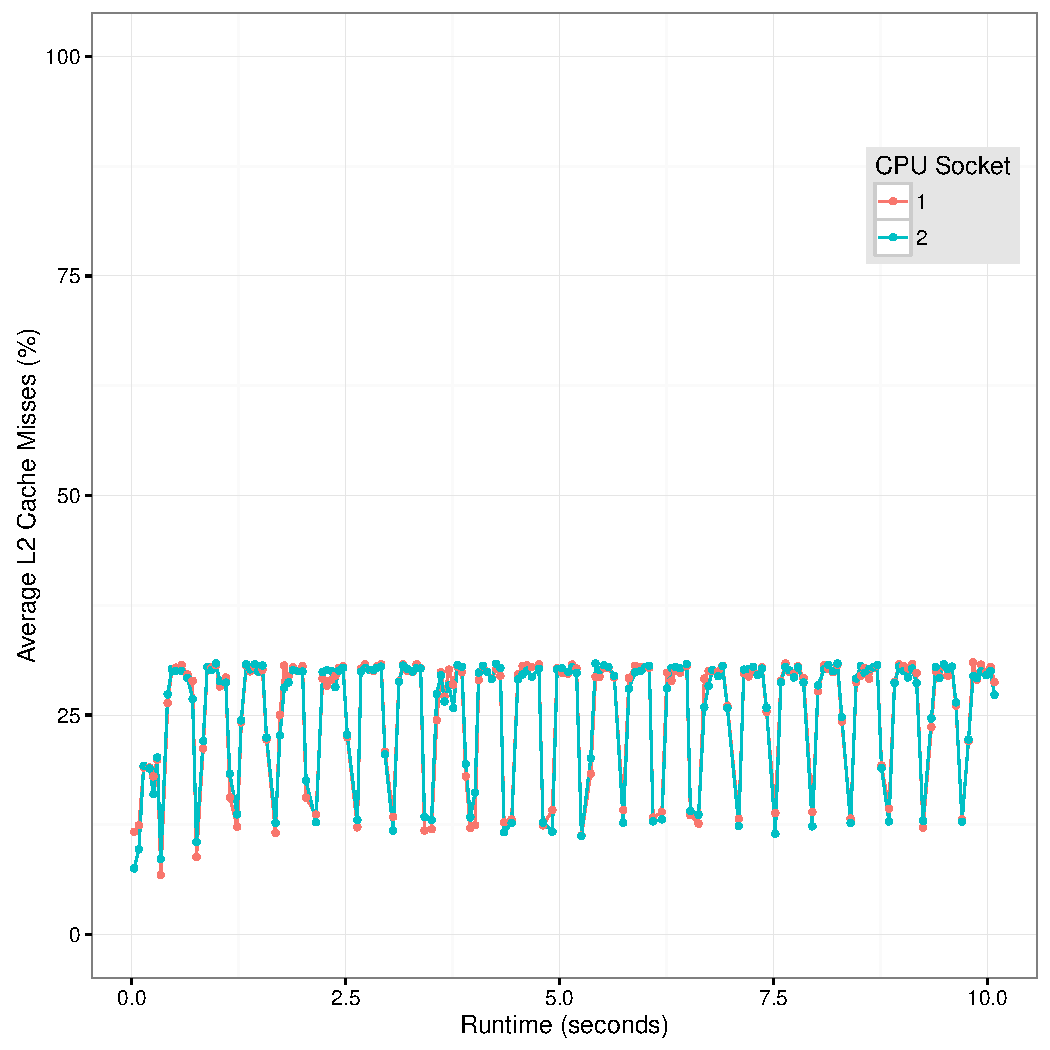
\includegraphics[width=8cm,height=8cm]{img/ftBNas_Analise.pdf}
\centering 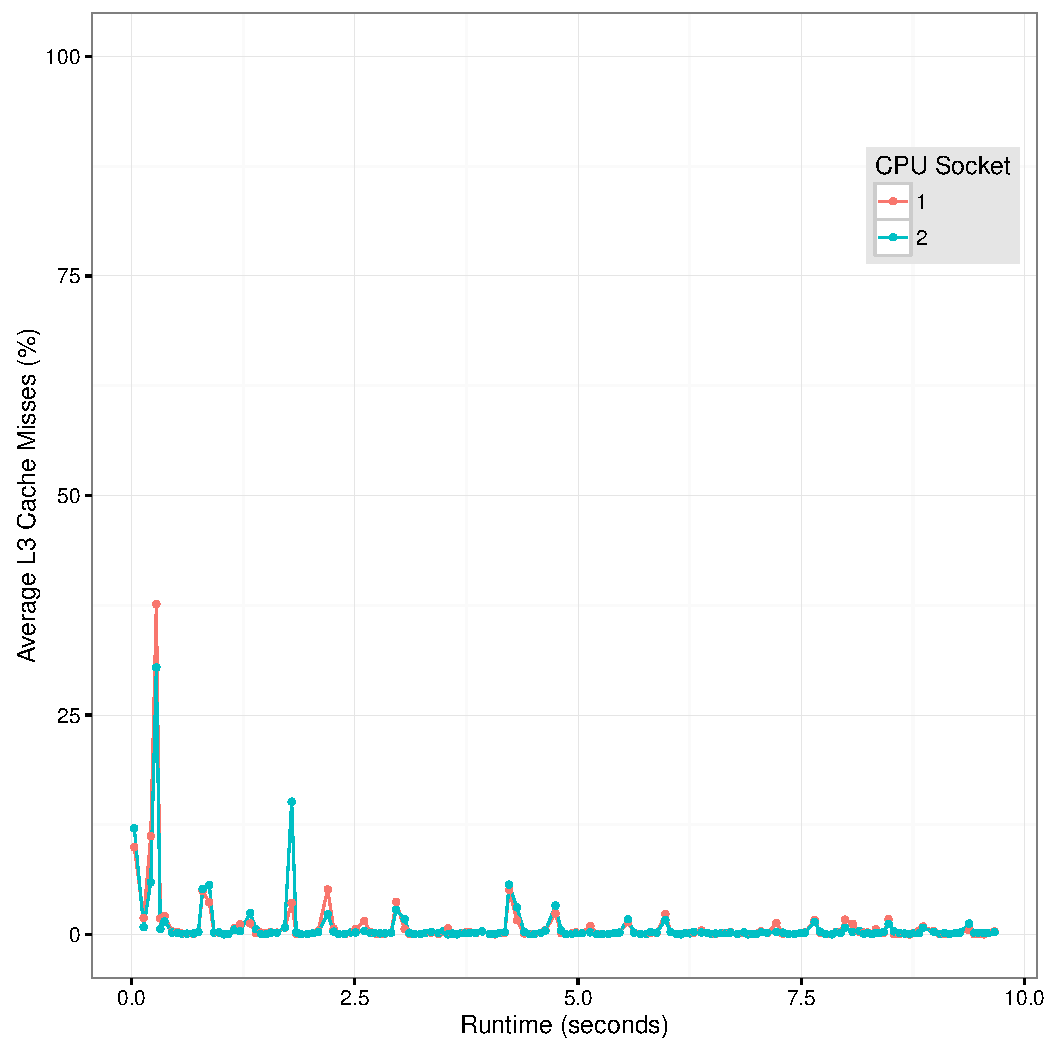
\includegraphics[width=8cm,height=8cm]{img/ftBNas_Analise_l3.pdf}
\caption{Execution of the Discrete 3D fast Fourier Transform.}
\end{figure}

The execution of the FT application (Figure x) shows that for the l2
cache there is a homogeneous behavior of the rate of misses during
execution of the application. The highest rate found in implementation
of FT was 31\% between 7.5 to 10 seconds late time execution. Already
the lowest rate was found about 6\% of missions in seconds of
execution. Regarding the behavior of the CPUs it is possible to see that
there is a closeness between the lines graphic, it may be related to
the application has a good load balancing between threads. Some points
have the disparity between the misses behavior of CPUs, as We are
analyzing the L2 cache level should take into account the
characteristic of the execution platform where the experiment was
executed, which is NUMA (Non-Uniform Memory Access to) and can
influence such behavior. 

Besides, it is possible can see that the application for the FT L3
cache level has a higher rate of misses equal to 37\% at the beginning
of the application. The higher rate of 37\% of the L3 cache misses may
be associated with the same timestamp occurred in the L2 cache, which
can be seen in the range of 0 to 2.5 seconds. The behavior of the miss
rate in the L3 cache is particular, the graph shows a linear range of
the different peaks where occurs more misses, the peaks will decrease
throughout the execution. Also, we visualize in this graph (as in the
L2 cache) that the two CPUs have a similar behavior.


\begin{figure}[htp]\label{figLU}
\centering 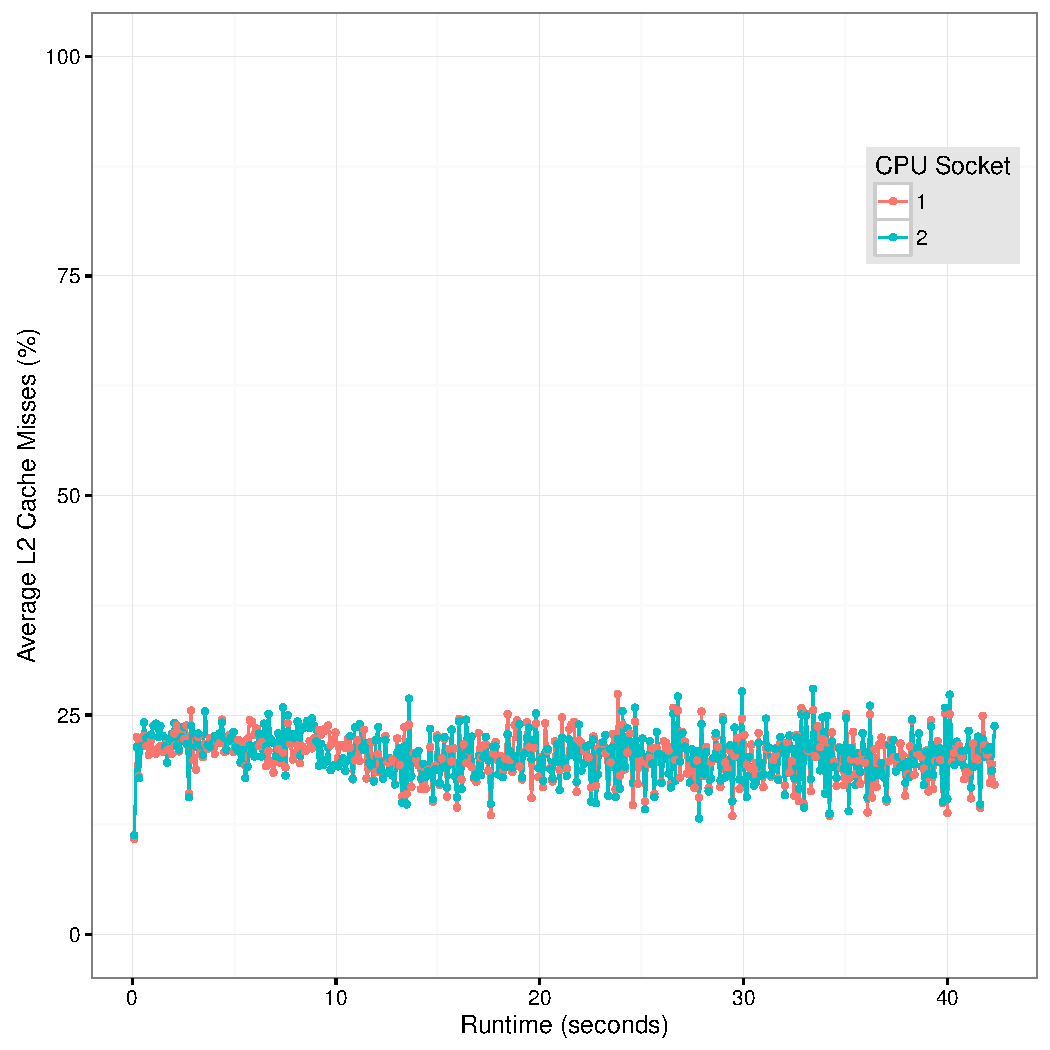
\includegraphics[width=8cm,height=8cm]{img/luBNas_Analise.pdf}
\centering 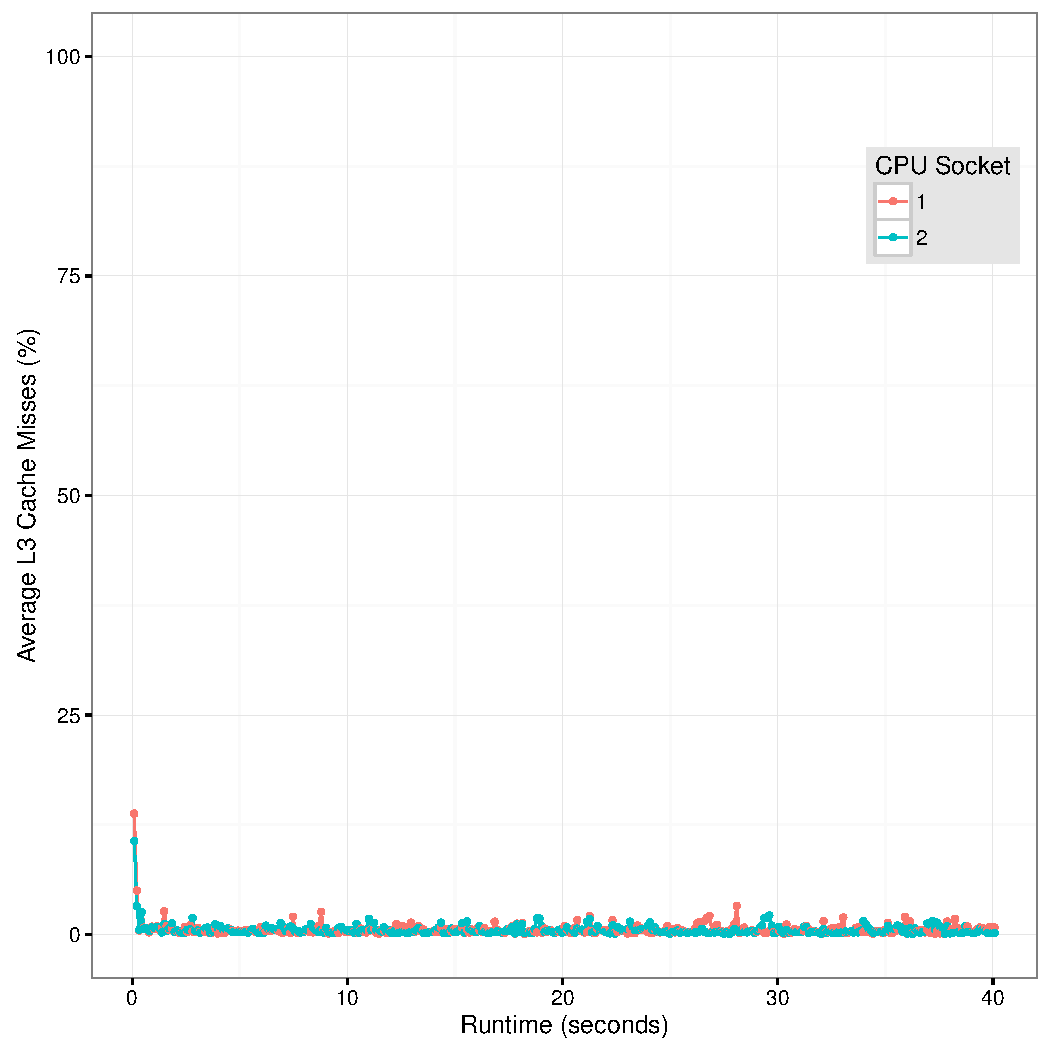
\includegraphics[width=8cm,height=8cm]{img/luBNas_Analise_l3.pdf}
\caption{Execution of the Lower-Upper Gauss-Seidel solver.}
\end{figure}

In the application LU it is possible to see that for the L2 cache, the
graph (Figure \ref{figLU}) has a more amorphous behavior, different from misses
behavior for the FT application (Figure \ref{figFT}). In some execution points,
CPUs have a different behavior in misses of the L2 cache. Most misses
rate in L2 for this application was 13\% in the first seconds of
running the application, already the lowest rate is less than 1\% and
occurs late in the range of 30 to 40 seconds of execution. 

The behavior of the LU application misses rate in the L3 cache has the
highest occurrence identified in the first seconds of execution, about
13\% of cache misses, the same timestamp that occurs first peak in
missions behavior in L2. Already identified the smallest rate was
about 0.07\% of misses after 36 seconds. The two CPUs had a more
similar behavior in this graphic can be observed a little difference
between their miss rates at the beginning of execution and also
between the range and 20 and 30 seconds.  

\begin{figure}[htp]\label{figCG}
\centering 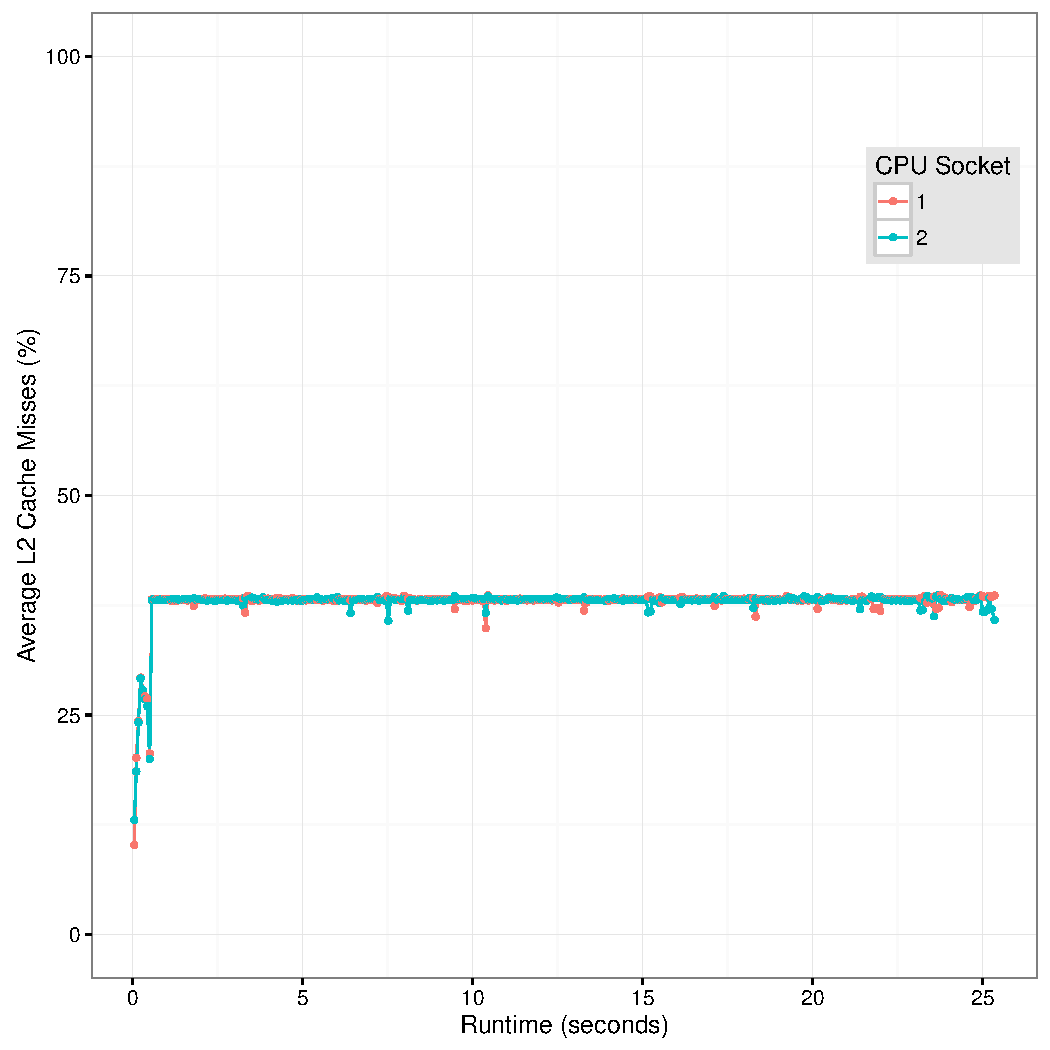
\includegraphics[width=8cm,height=8cm]{img/cgBNas_Analise.pdf}
\centering 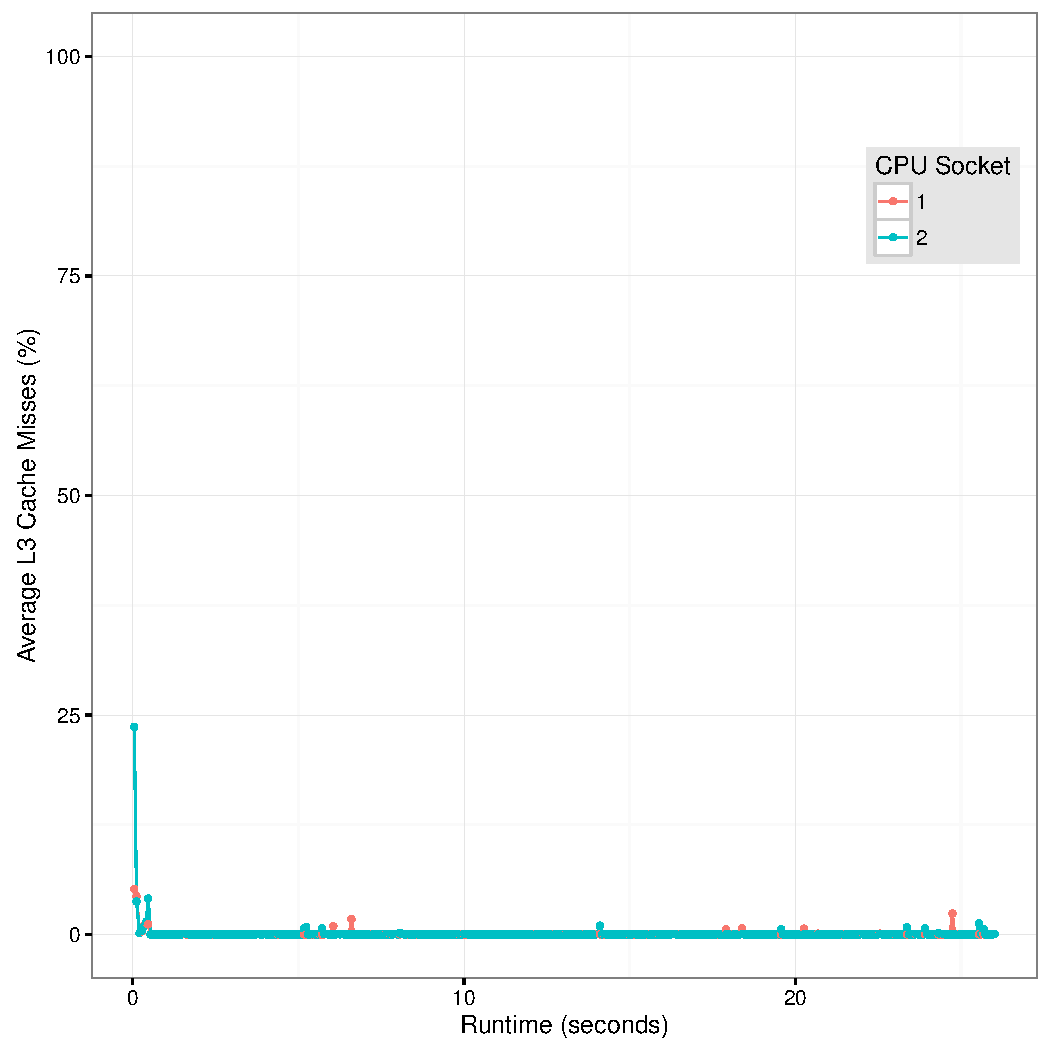
\includegraphics[width=8cm,height=8cm]{img/cgBNas_Analise_l3.pdf}
\caption{Execution of the Conjugate Gradient.}
\end{figure}


Figure \ref{figCG} shows the misses rate for CG application in L2 cache, it is
possible to see that at the beginning of implementation there is a
considerable increase in cache misses rate after this peak rate
remains linearly. The highest value was identified for when the
application reached 23 seconds of execution, about 38\% higher value
than other applications for L2 cache, which may be related to the
application characteristics, which has irregular access memory,
different from other applications. The lowest index cache misses was
identified earlier in the application, about 10\%. As for the L3 cache,
it is possible to identify an increase in cache misses rate at the
beginning of the application, about 23\% after its behavior is linear.

\section{Conclusion}
\label{sec:orgheadline5}
\label{sec:conclusion}


The results show cache misses rate results for the L2 cache and also
to the L3 cache. From this result, it is possible to define the most
memory-bound regions, which have a rate of cache misses larger than
the other, as well as more CPU-bound regions that have smaller cache
misses rates. In our experiment, where were performed the FT
applications (3D Discrete Fast Fourier Transform), LU (Lower-Upper
Gauss-Seidel solver) and Conjugate Gradient (CG) is possible see which
applications are more memory-bound than the other and in which parts
of its execution, they are more memory-bound.

Not all tools offer adequate support to collect counters in hardware
small time intervals (msec range), the tool used (likwid) provided the
values of the respective counters hardware of time slices requested
timestamp defined in the experiments, allowing examine other
characteristics to define memory-bounds areas of a parallel
application. 

The next step of the work consists of the following steps: explore
other measures to define with greater accuracy the memory-bound
regions, align the technique of Design of Experiments in our
methodology and use the DVFS application for efficiency energy and
higher performance for applications specifically identified in the
parallel memory-bound regions. 


\section*{Acknowledgements}

This research receives HPC-ELO project funds, the H2020
program EU and MCTI / RNP-Brazil through HPC4E project
with code 689772

%Who paid for this?

\bibliographystyle{IEEEtran}
\bibliography{refs}
\end{document}